\section{Why?}

AXI4-Stream is intended to be used on a MicroBlaze-Embedded-System, in order to send/receive data over an IP core. Therefore, the following system in figure~\ref{f0} will be used as reference  design for this documentation. Moreover, the main goal of this documentation is to provide essential knowledge to adapt or create IP-cores to work with AXI4-Stream in a MicroBlaze-Embedded-System. Additionally, extra functionality to the interface is added beside the communication interface itself. For example, a reset output that can be controlled by software. Thus, users could be able to reset their system easily. All these details will be covered in later sections.

\begin{figure}[!h]
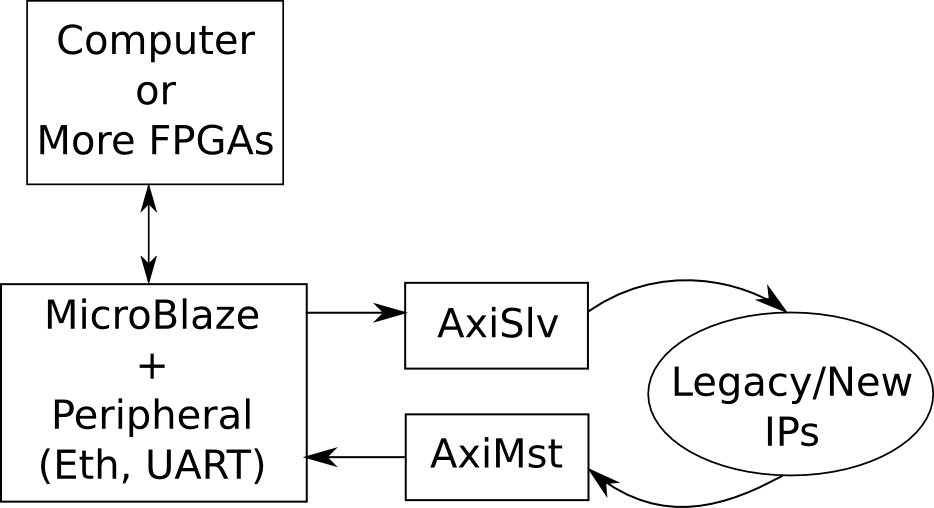
\includegraphics[scale=0.35]{images/idea.png}
\caption{Microblaze Embedded System.}
\label{f0}
\end{figure}

